\documentclass[12pt]{article}
\usepackage{cite}
\usepackage{graphicx}
\usepackage{geometry}
\usepackage{float}
\usepackage{multicol}

\geometry{left=2.0cm,right=2.0cm,top=2.5cm,bottom=2.5cm}

\title{
    \textbf{\Huge ECE385} \\
    \huge Fall 2020 \\
    \huge Experiment 1 \\[120pt]
    \textbf{\Huge Introductory Experiment} \\[120pt]
    }

\author{
    \large Name: Zhang Yichi \\
    \large Lab Section: LA3 \\
    \large TA's Name: Yu Yuqi
    }

\date{Sept. $16^{th}\quad$ 2020}

\begin{document}
\maketitle
\newpage

\section{Introduction}
\subsection{\textbf{Purpose of Circuit}}
The purpose of this lab is to build a two to one multiplexer (mux) which allows us to select the signals we want. A two to one mux uses an one digital signal to select one of the two input signals to be the output signal. Using the same principle, much more complicated muxes could be built. With $n$ signals, we can select one output signal from $2^n$ input signals. This can be used later in the memory to select the correct unit corresponding to the desired address. \\

\noindent
Another prupose of this lab is to show the static hazard. In ECE120, we choose to ignore certain aspects of circuit design to emphasize a strong theoretical base for further study \cite{GG}, e.g. the static hazard. However, in this lab, it will be no longer ignored. We will observe the static hazard, analyze the reason why it happens and try to eliminate it.

\section{Documentation}
\subsection{\textbf{Written Description of Circuit}}
There are three input signals A, B and C in our circuit. A and C are the potential output signals. B is the signal to select which one is the output. All of them form a two to one mux. Use $Z$ to denote the output, then $Z=AB+B'C$ in part A. However, in this way, the inverter will create a delay and cause static hazard. To eliminate it, we add a new combination term of input, $AC$, in part B which makes the output $Z=AB+B'C+AC$. In this case, with $AC=1$, whenever $B$ switches from 0 to 1 or 1 to 0, the $AC$ term will continuously give the output an 1 to make it stable at 1. Detailed illustration will be presented as timing diagram in the Documentation part.
\begin{figure}[H]
    \centering
    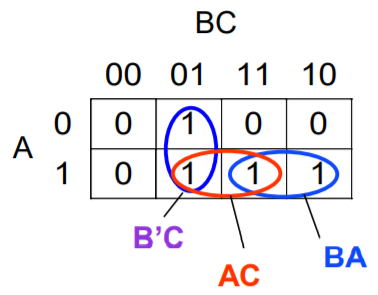
\includegraphics[scale=0.5]{K_map.png}
    \caption{K-map for the theoretical principle. The blue circle is for part A and the red circle is for the added term $AC$ in part B \cite{PPT}.}
\end{figure}


\subsection{\textbf{Logic Diagrams}}
\begin{figure}[H]
    \centering
    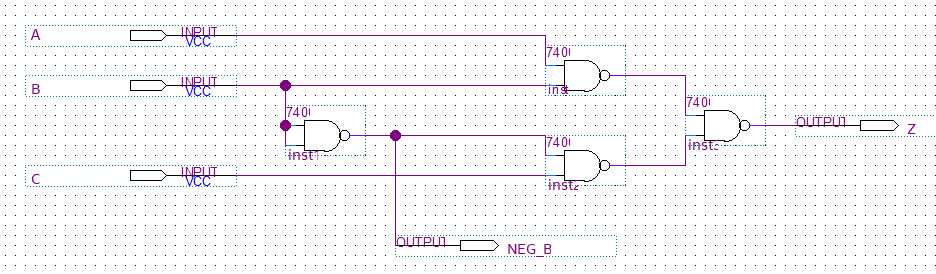
\includegraphics[scale=0.7]{lab1_partA.png}
    \caption{Circuit of part A without DELAY module}
\end{figure}

\begin{figure}[H]
    \centering
    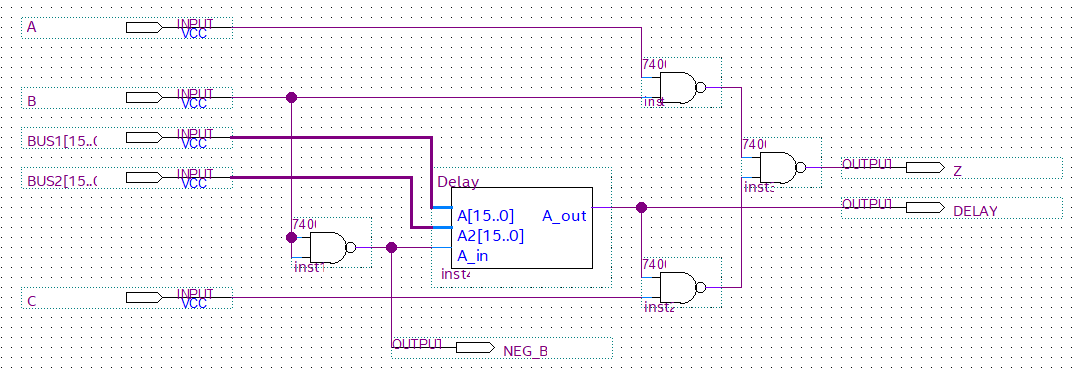
\includegraphics[scale=0.5]{lab1_partADelay.png}
    \caption{Circuit of part A with DELAY module}
\end{figure}

\begin{figure}[H]
    \centering
    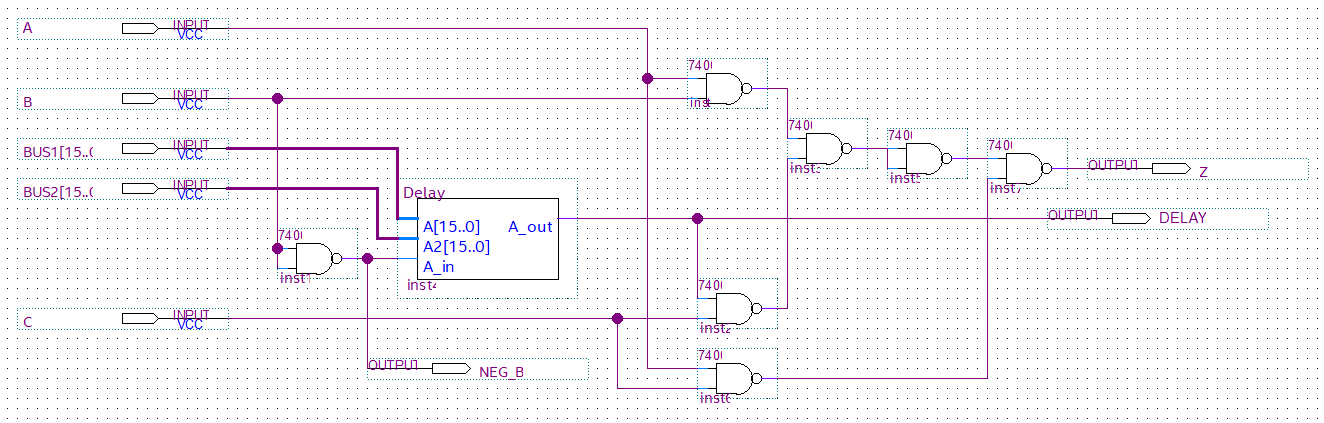
\includegraphics[scale=0.4]{lab1_partB.png}
    \caption{Circuit of part B}
\end{figure}

\subsection{\textbf{Annotated Simulation Waveform}}
\begin{figure}[H]
    \centering
    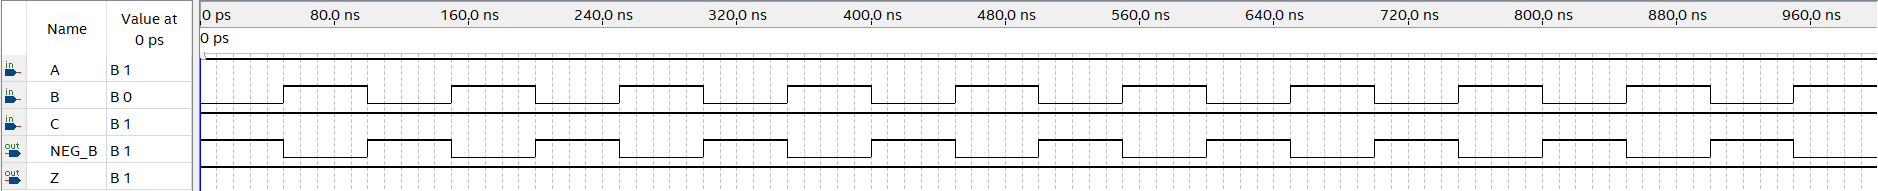
\includegraphics[width=18cm]{lab1_partA_func_sim.png}
    \caption{Waveform of part A by functional simulation. No delay considered.}
\end{figure}

\begin{figure}[H]
    \centering
    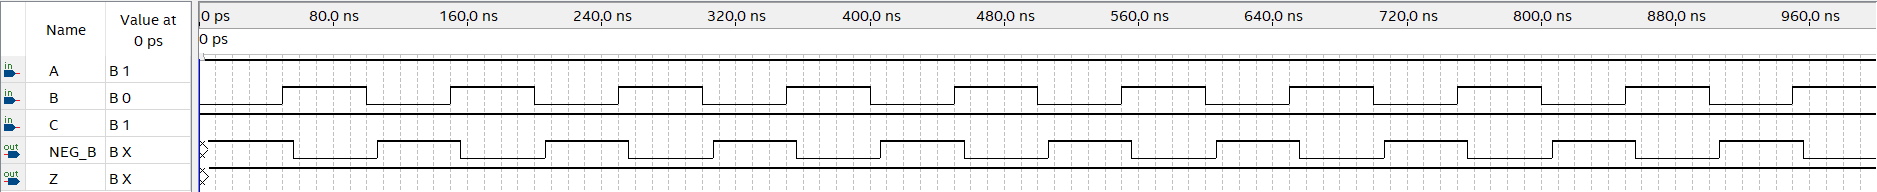
\includegraphics[width=18cm]{lab1_partA_waveform.png}
    \caption{Waveform of part A without DELAY module. Inverter create a small delay at the beginning but too small to cause obvious glitch in $Z$ to show the static hazard.}
\end{figure}

\begin{figure}[H]
    \centering
    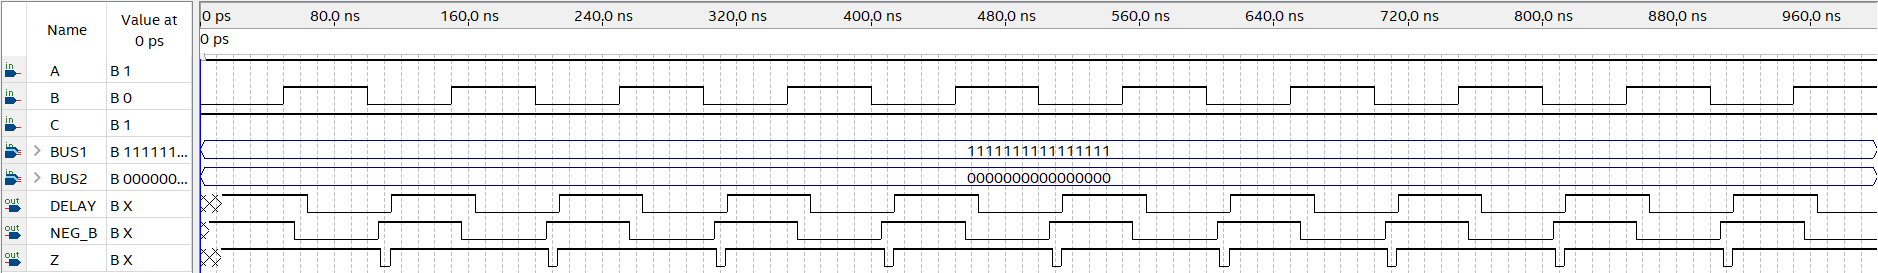
\includegraphics[width=18cm]{lab1_partADelay_waveform.png}
    \caption{Waveform of part A with DELAY module. DELAY module highly increases the delay after the inverter which makes it now long enough to cause obvious glitch in $Z$ to show the static hazard.}
\end{figure}

\begin{figure}[H]
    \centering
    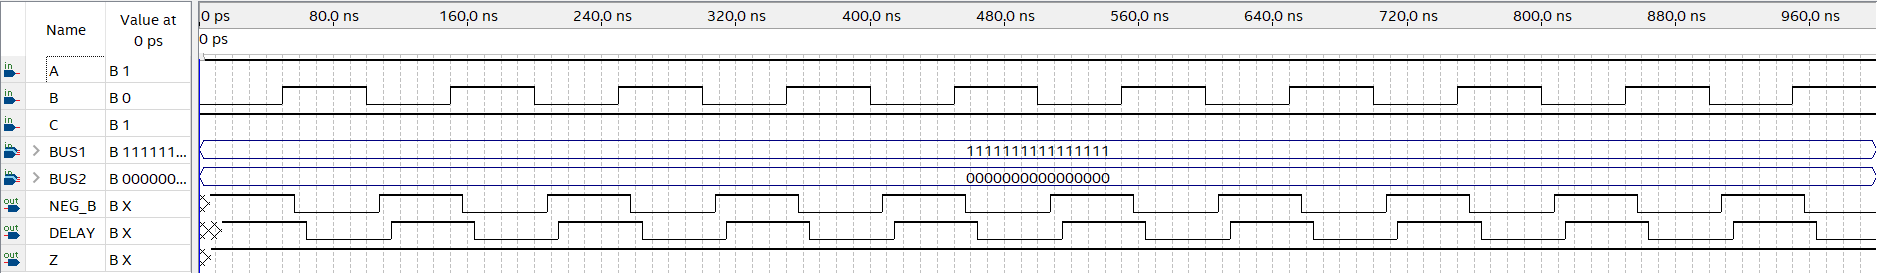
\includegraphics[width=18cm]{lab1_partB_waveform.png}
    \caption{Waveform of part B. Adding the $AC$ term to the circuit, the long delay still exists as the DELAY output shows, but the glitch in $Z$ disappears which means the static hazard is successfully eliminated.}
\end{figure}

\subsection{\textbf{Truth Table}}
\begin{figure}[H]
    \centering
    \begin{table}[H]
        \centering
        \resizebox*{5cm}{8cm}{
            \begin{tabular}{|l|l|l|l|}
                \hline
                A & B & \multicolumn{1}{c|}{C} & Z \\ \hline
                0 & 0 & 0                      & 0 \\ \hline
                0 & 0 & 1                      & 1 \\ \hline
                0 & 1 & 0                      & 0 \\ \hline
                0 & 1 & 1                      & 0 \\ \hline
                1 & 0 & 0                      & 0 \\ \hline
                1 & 0 & 1                      & 1 \\ \hline
                1 & 1 & 0                      & 1 \\ \hline
                1 & 1 & 1                      & 1 \\ \hline
            \end{tabular}
        }
    \end{table}
    \caption{Truth table for both part A ($Z=AB+B'C$) and part B ($Z=AB+B'C+AC$).}
\end{figure}

\section{Answers}
\subsection{\textbf{Answers to Pre-Lab Questions}}
Question: No groups may observe static hazards. Why? If you do not observe a static hazard, chain an odd number of inverters together in place of the single inverter from Figure 16. But no static hazard is find, why? Wait for class and I will tell you. \\

\noindent
Answer: Functional simulation is an ideal simulation. It calculates the final output directly from the input without considering any delay. Time simulation considers the delay but we still cannot see the static hazard because the delay of an inverter is too small to cause obvious glitch to show the static hazard. Chaining an odd number of inverters to increase the delay also failed because the Quartus automatically optimize the circuit to make it counts only one inverter's delay. \\

\subsection{\textbf{Answers to Lab Questions}}
Question: Test the circuit of part A of the pre-lab by using waveform editor, simulate with Functional simulation. Complete a truth table of the output as a function of the three inputs. \\

\noindent
Answer: Function simulation, see Fig. 4 in Documentation 2.3. Truth table, see Fig. 8 in Documentation 2.4. \\

\noindent
Question: Test the circuit in part B of the pre-lab, including Delay module as well. Complete a truth table of the output. Does it respond like the circuit of part A? Describe and save the output and explain any differences between it and the results obtained in part 2. Consider the following question and explain: for the circuit of part A of the pre-lab, at which edge (rising/falling) of the input B are we more likely to observe a glitch at the output? \\

\noindent
Answer: Truth table, see Fig. 8 in Documentation 2.4. Yes, the static hazard is eliminated. At the \textbf{falling} edge (1 to 0), it is more likely for us to observe a glitch because when B turns from 1 to 0, the $B'C$ term will not be 1 immediately since there is a delay for the inverter which means there will be 2 gates delay. However, when B turns from 0 to 1, the $AB$ term can turn to 1 after only 1 gate delay. \\

\subsection{\textbf{Answers to Post-Lab Questions}}
Question: How long does it take the output Z to stabilize on the falling edge of B (in ns)?  How long does it take on the rising edge (in ns)? Are there any potential glitches in the output, Z? If so, explain what makes these glitches occur. \\

\noindent
Answer: It takes 60 ns for the output Z to stabilize on the falling edge and the same on the rising edge. The potential glitches will happen during the two 60 ns. When B changes from 0 to 1 or 1 to 0, there will be two unstable time zones and static hazards might happen at these time.

\begin{figure}[H]
    \centering
    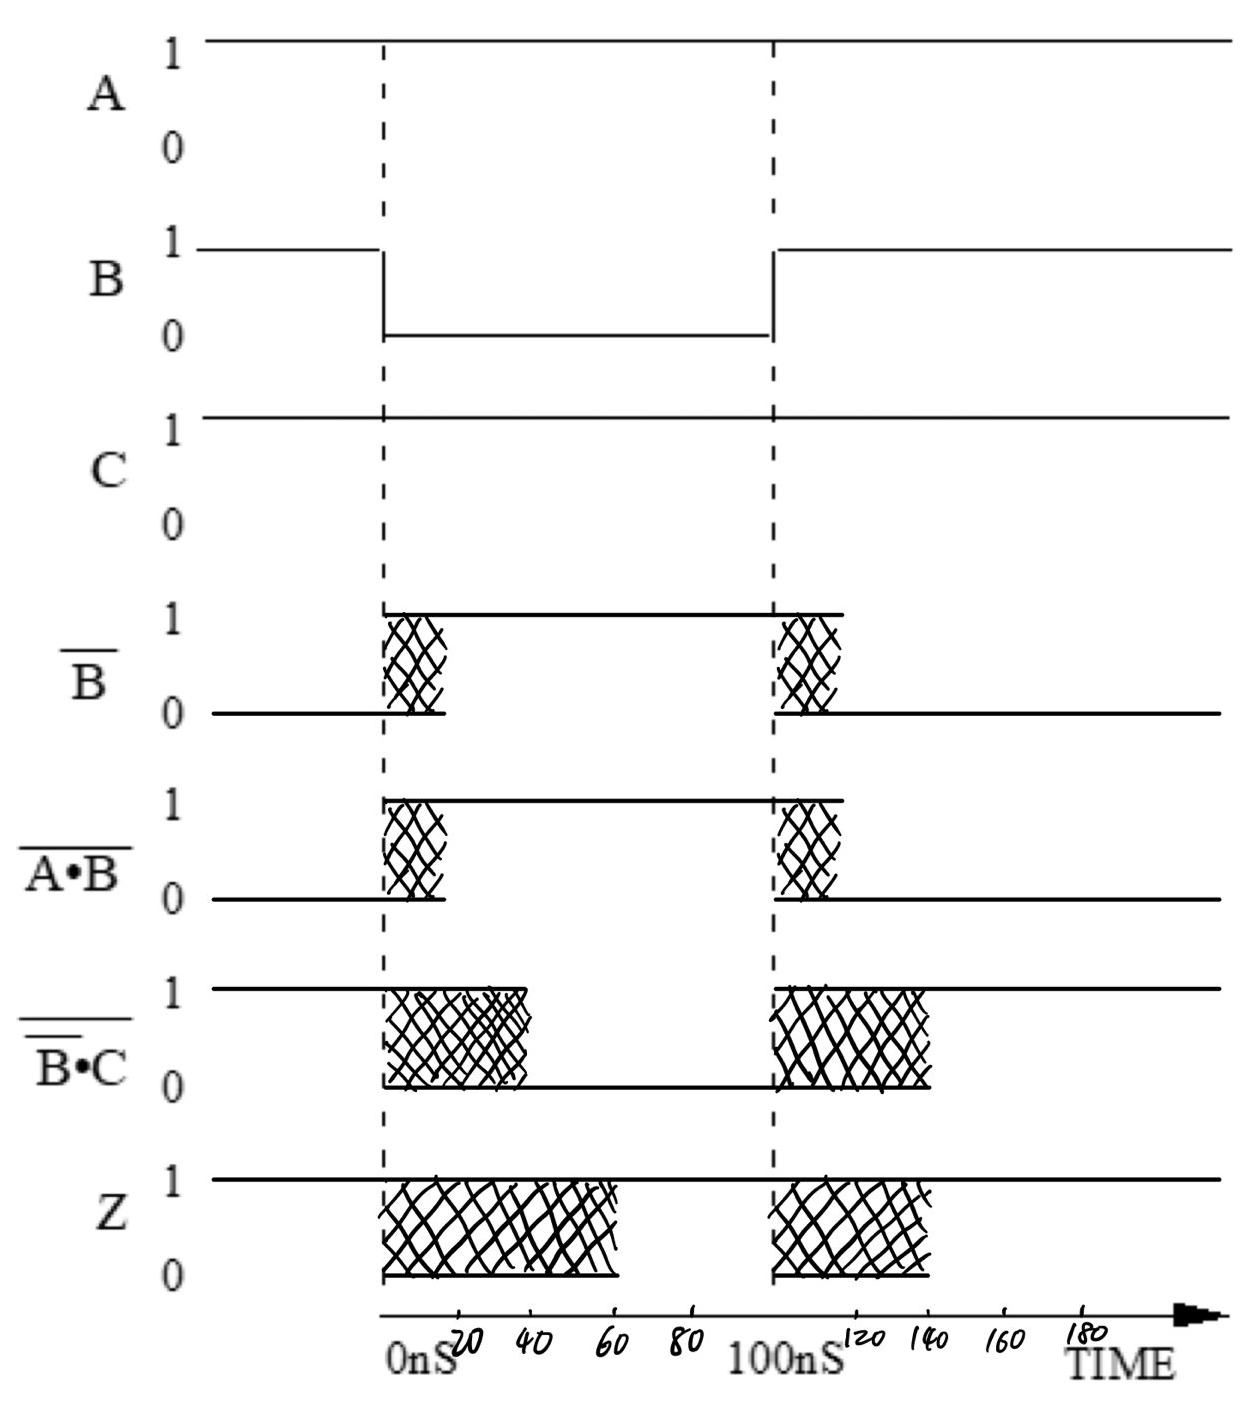
\includegraphics[scale=0.25]{timing_diagram.png}
    \caption{Timing diagram}
\end{figure}

\subsection{\textbf{Answers to questions from the General Guide}}
GG.6: What is the advantage of a larger noise immunity? Why is the last inverter
observed rather than simply the first? Given a graph of output voltage (VOUT) vs. input voltage (VIN) for an inverter, how would you calculate the noise immunity for the inverter? \\

\noindent
Answer: Larger noise immunity means higher stability. If the input is noisy, the chip can still work. Only one inverter is not able to show the stability, so we use a series of inverters to amplify the noise (instability) to give us a reliable nominal range. To calculate the noise immunity of Y, we subtract the lowest input voltage that would result in low level output from the high level output voltage. To calculate the noise immunity of X, we subtract the low level output voltage from the highest input voltage that would result in high level output. Then to get the overall noise immunity, we take the smaller one from the noise immunity of X and Y. \\

\noindent
GG.29: If we have two or more LEDs to monitor several signals, why is it bad practice to share resistors?

\noindent
Answer: Different LEDs have different forwarding bias even with same kinds (colors) of LEDs. Thus, sharing a resistor will make some of the LEDs brighter and some dimmer. Sometimes it can be dangerous or even blow up if one LED is too bright (getting too much current going through).

\section{Conclusion}
This is an introductory experiment. We build a mux and learn to eliminate static hazards which were ignored before in ECE120 but really worth paying attention to. Also, this is the first time we do simulation on the software, Quartus. We are free to debug and find out which element is broken but now trapped in solving why the compiling failed and why the simulation failed. In all, it is a good transition from ECE120 to ECE385.

\newpage
\bibliography{lab1_ref}
\bibliographystyle{ieeetr}
\end{document}